\documentclass{gescons}

\genre {Entrevista}
\author{Pedro Borges}
\title{Eitologia: Teática Inversiva}
\paginaurl{https://www.youtube.com/live/eSvrYKBw43c}

\begin{document}
    \makeentrevistatitle
    \coverart{back/Pedro_Borges}

    \begin{multicols}{2}

\begin{center}
    \vspace{-1cm}
    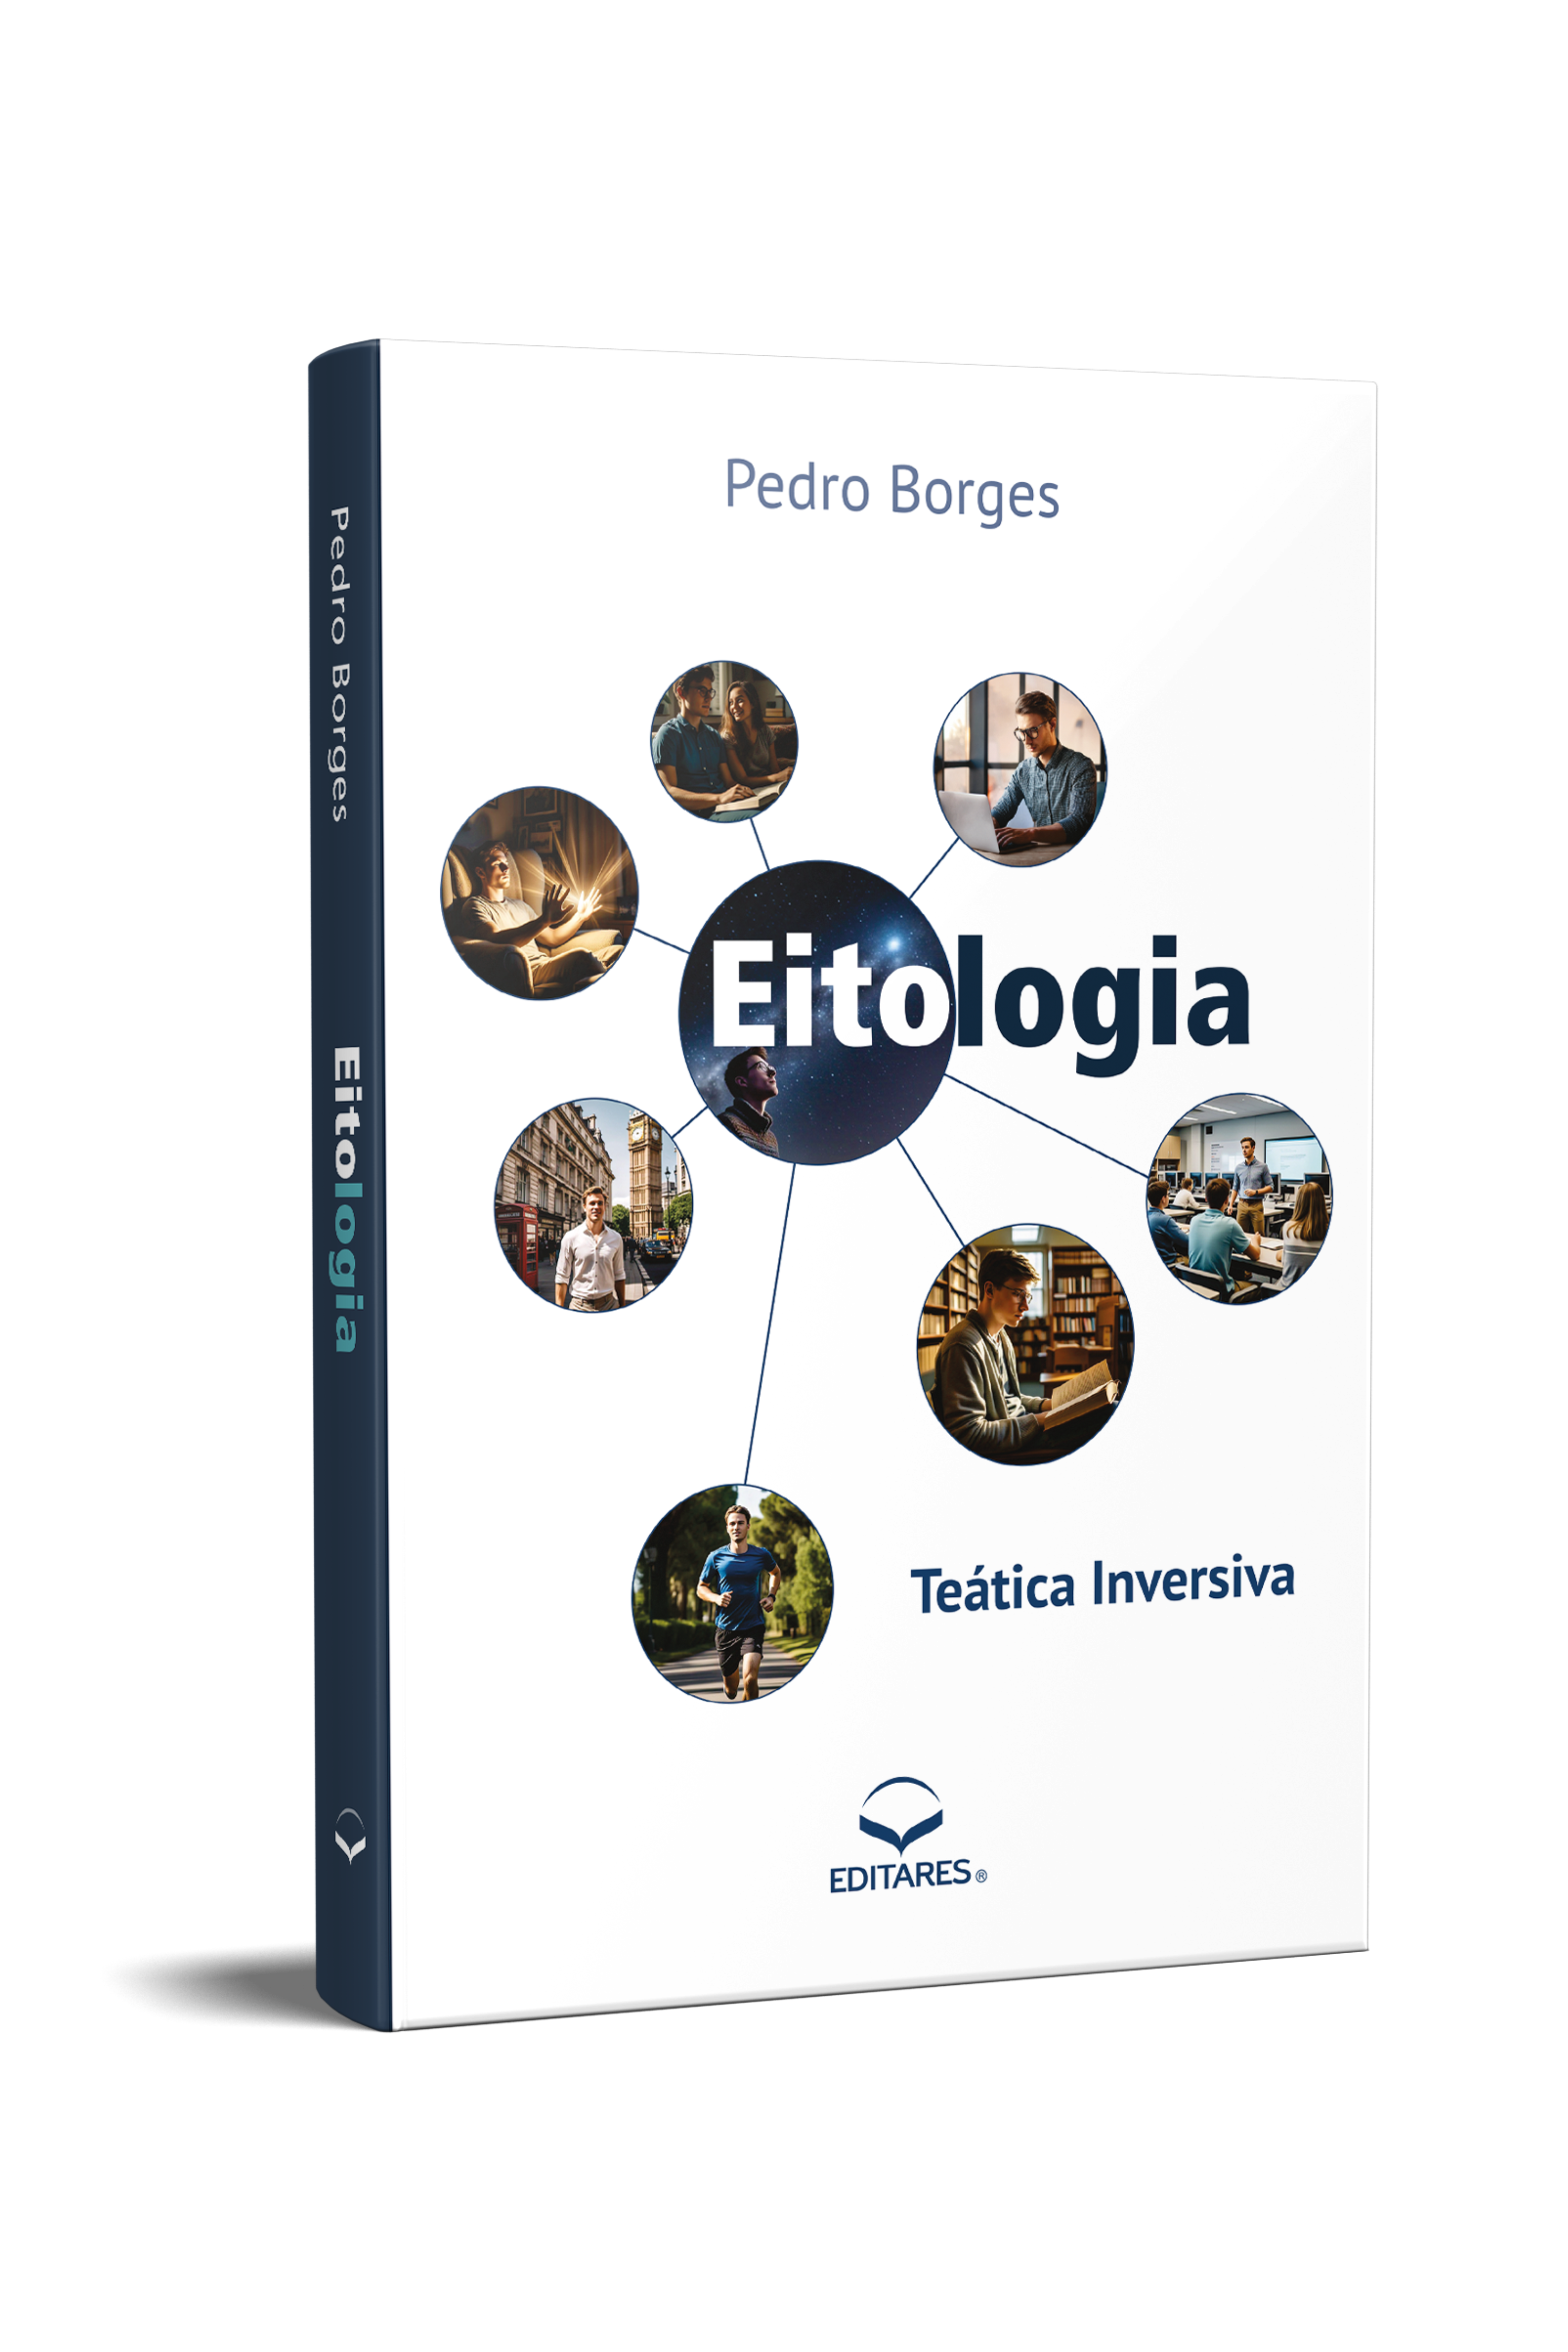
\includegraphics[width=6cm]{articles/entrevista/mockups/Pedro_Borges.png}
\end{center}

\vspace{-1cm}

\subsubsection{1.       Qual foi a~motivação para a~escrita da obra? Por que a~definição deste tema para publicação de um livro?}

A motivação foi compreender melhor como conduzir as várias frentes da vida humana em conjunto e~sempre em frente, mapeando o~fluxo existencial do intermissivista ao assumir o~desafio de vivenciar o~pacote completo da Conscienciologia.

Para isso, valer-se de uma técnica evolutiva, no meu caso a~inversão existencial, enquanto ferramenta para organização pessoal em prol da dinamização lúcida da evolução, é~algo que ajuda bastante a~concentrar o~exclusivismo dos interesses pessoais na assistencialidade de modo mais otimizado.

A definição do tema enquanto Eitologia foi a~forma mais eficaz e~chamativa encontrada para se estudar a~postura, atitude ou comportamento de levar tudo de eito, expressão coloquial bastante utilizada pelo prof. Waldo Vieira em suas aulas, debates e~atendimentos, enquanto princípio fundamental para realização atacadista, a~maior, da programação existencial, sem deixar nada para trás.

\subsubsection{2.       Quais foram as principais percepções, intra e~extrafísicas, durante a~pesquisa e~a~escrita da obra? E~posterior ao lançamento?}

A motivação foi compreender melhor como conduzir as várias frentes da vida humana em conjunto e~sempre em frente, mapeando o~fluxo existencial do intermissivista ao assumir o~desafio de vivenciar o~pacote completo da Conscienciologia.

Para isso, valer-se de uma técnica evolutiva, no meu caso a~inversão existencial, enquanto ferramenta para organização pessoal em prol da dinamização lúcida da evolução, é~algo que ajuda bastante a~concentrar o~exclusivismo dos interesses pessoais na assistencialidade de modo mais otimizado.

% \begin{pullquote}
%     ``O que vai para o~papel é~uma expressão direta da consciencialidade do autor.''
% \end{pullquote}


\subsubsection{3.       Qual o~maior aprendizado com a~escrita desta obra?}

Complementando o~que foi comentado na questão anterior, um dos grandes aprendizados foi o~de verificar na prática o~quanto a~escrita de um livro conscienciológico é~conscienciográfica, pois o~que vai para o~papel é~uma expressão direta da consciencialidade do autor, sendo de grande relevância para a~obra fazer sentido à~própria verbação perante o~que se deixou grafado.


\subsubsection{4.       O~que poderia dizer como incentivo para que mais pesquisadores invistam na publicação de obras conscienciológicas?}

Escolha uma temática de interesse, busque bibliografia em todas as bases de consulta da Conscienciologia e~comece a~focar naquele assunto. Busque convergir as atividades para aquela temática, anote as experiências. Antes de começar a~escrever, defina o~escopo, a~estrutura do livro e~o~público-alvo. E~busque assessoria da Uniescon. Há várias atividades na IC para ajudar o~autorando. 
    
Levar tudo de eito envolve não deixar nada para trás, e~um dos pontos mais sérios desta condição é~a~publicação de obra conscienciológica, pois aciona um ponto de convergência entre várias áreas da vida, mexendo com a~consciência como um todo. Nesse sentido, para o~livro sair redondo, precisa-se desenvolver, não só a~intelectualidade, mas também o~parapsiquismo, a~autopesquisa, a~vida financeira, a~parte afetiva, a~liderança no voluntariado, entre outras variáveis. Tanto quem tem facilidade em escrever possui responsabilidade de compartilhar os achados pesquisísticos com teática, quanto aqueles que sentem dificuldade em colocar no papel possuem hoje condições de superar este travão e~materializar a~obra, com todos os recursos disponíveis na CCCI, ao modo de assessorias, cursos e~editora especializada. Não desperdice, aproveite!

    \end{multicols}
\end{document}
